\documentclass[tikz,border=3pt]{standalone}
\usepackage[utf8]{inputenc}
\usepackage[T1]{fontenc}
\usepackage{lmodern}
\renewcommand{\familydefault}{\sfdefault}
\usepackage{sansmath}\sansmath
\usepackage{chemfig}
\usepackage{pgfplots}\pgfplotsset{compat=1.18,/pgf/number format/use comma,/pgf/number format/1000 sep={.}}
\usetikzlibrary{arrows.meta,calc,positioning,decorations.pathmorphing,patterns}
% paleta del sitio
\definecolor{nar}{HTML}{E8680C}\definecolor{narc}{HTML}{FFB35C}\definecolor{hielo}{HTML}{FFF3E8}
\definecolor{tinta}{HTML}{1D1D1F}\definecolor{gris}{HTML}{6E6E73}\definecolor{lila}{HTML}{7C5CF0}
\definecolor{azul}{HTML}{2F6FD6}\definecolor{menta}{HTML}{17A673}\definecolor{coral}{HTML}{E8342A}
\begin{document}
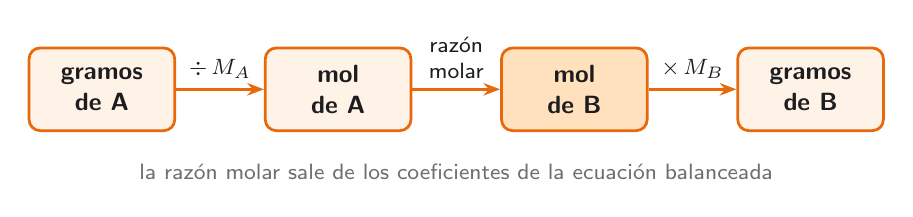
\begin{tikzpicture}
\tikzset{caja/.style={draw=nar,fill=hielo,line width=1pt,rounded corners=4pt,minimum width=1.85cm,minimum height=1.05cm,align=center,font=\sffamily\small\bfseries,text=tinta},
  fl/.style={-{Stealth[length=6pt]},line width=1.1pt,nar},et/.style={font=\sffamily\footnotesize,text=tinta,align=center}}
\node[caja] (a) at (0,0) {gramos\\de A};
\node[caja] (b) at (3,0) {mol\\de A};
\node[caja,fill=narc!40] (c) at (6,0) {mol\\de B};
\node[caja] (d) at (9,0) {gramos\\de B};
\draw[fl] (a) -- node[et,above] {$\div\, M_A$} (b);
\draw[fl] (b) -- node[et,above] {razón\\molar} (c);
\draw[fl] (c) -- node[et,above] {$\times\, M_B$} (d);
\node[font=\sffamily\footnotesize,text=gris] at (4.5,-1.05) {la razón molar sale de los coeficientes de la ecuación balanceada};
\end{tikzpicture}
\end{document}
